\section{Measurement, Uncertainty, and Variation\footnote{
1990-93 Dept. of Physics and Astronomy, Dickinson College. Supported by FIPSE
(U.S. Dept. of Ed.) and NSF. Portions of this material may have been modified
locally and may not have been classroom tested at Dickinson College.
}}

\makelabheader %(Space for student name, etc., defined in master.tex or labmanual_formatting_commands.tex)

\bigskip
\textbf{Objectives }

\begin{itemize}[nosep]
\item To explore the mathematical meaning of the standard deviation and standard error
associated with a set of measurements. 
\item To investigate random and systematic variations associated with a set of measurements.
\end{itemize}

\bigskip
\textbf{Statistics - The Inevitability of Uncertainty }

With care and attention, it is commonly believed that both mistakes and systematic
errors can be eliminated completely. However, inherent uncertainties do not
result from mistakes or errors. Instead, they can be attributed in part to the
impossibility of building measuring equipment that is precise to an infinite
number of significant figures. The ruler provides us with an example of this.
It can be made better and better, but it always has an ultimate limit of precision.

Another cause of inherent uncertainties is the large number of random variations
affecting any phenomenon being studied. For instance, if you repeatedly drop
a baseball from the level of the lab table and measure the time of each fall,
the measurements will most probably not all be the same. Even if the stop watch
was gated electronically so as to be as precise as possible, there would be
small fluctuations in the flow of currents through the circuits as a result
of random thermal motion of atoms and molecules that make up the wires and circuit
elements. This could change the stop watch reading from measurement to measurement.
The sweaty palm of the experimenter could cause the ball to stick to the hand
for an extra fraction of a second, slight air currents in the room could change
the ball's time of fall, vibrations could cause the floor to oscillate up and
down an imperceptible distance, and so on.

\bigskip
\textbf{Repeated Time-of-Fall Data} 

In the first two activities, you and your partners will take repeated data on
the time of fall of a ball and study how the data vary from some average value
for the time-of-fall.

\textbf{Apparatus} 

\begin{itemize}[nosep]
\item A ball 
\item A stop watch 
\item A 2-meter stick
\end{itemize}

\bigskip
\textbf{Activity 1: Timing a Falling Ball} 

(a) Drop the ball so it falls through a height of exactly 2.0 m at least 10
times in rapid succession and measure the time of fall in each case. Be as exact as possible about the height from which you drop the ball. Record your 10 time values here:
\answerspace{40mm}

\pagebreak[2]
(b) Enter your data as a single column in Excel and find the 
average (mean) of the data.
See \textbf{Appendix \ref{excel}} for instructions. Report the
mean value in the space below (including units).
\vspace{10mm}

\textbf{The Standard Deviation as a Measure of Uncertainty }

How certain are we that the average fall-time determined in the previous activity
is accurate? The average of a number of measurements does not tell the whole
story. If all the times you measured were the same, the average would seem to
be very precise. If each of the measurements varied from the others by a large
amount, we would be less certain of the meaning of the average time. We need
criteria for determining the certainty of our data. Statisticians often use
a quantity called the standard deviation as a measure of the level of uncertainty
in data. The standard deviation is usually represented by the Greek letter \( \sigma  \)
(sigma). A customary way of expressing an experimentally determined value is:
Mean  \( \pm \ \sigma  \). The formal mathematical definition of \( \sigma  \)
can be found in \textbf{Appendix \ref{treatment}}.

In the next activity you will use Excel (see \textbf{Appendix \ref{excel}}) to calculate
the value of the standard deviation for the repeated fall-time data you just
obtained and explore how the standard deviation is related to variation in your
data. In particular, you will try to answer this question: What percentage of
your data lies within one standard deviation of the average you calculated?

\textbf{Activity 2: Standard Deviation} 

(a) Report the value for the standard deviation of your data in the space below (including units).
\answerspace{10mm}

(b) In the space below, write the time of fall from your data as $t$ = \(\langle t\rangle 
\pm  \sigma  \), (including units).
\answerspace{10mm}

(c) Determine the number of your data points that lie within \( \pm  \sigma  \)
of the average and write the result in the space below. Also, calculate the
percentage of data points lying within a standard deviation of the average and
report that result.
\answerspace{10mm}

(d) Combine your results with those obtained by the other groups in the class
and create a table in the space below with the following column headings: Lab
Station, \( \langle t\rangle\) (s), \( \sigma  \) (s), \%Data \( \pm \sigma  \).
\answerspace{40mm}

(e) Study the last column, which represents the percentage of data points lying
within one standard deviation of the average. What does the standard deviation,
\( \sigma  \), tell you about the approximate probability that another measurement
will lie within \( \pm \sigma  \) of the average?
\answerspace{15mm}

\pagebreak[2]
\textbf{Systematic Error - How About the Accuracy of Your Timing Device and
Timing Methods?} 

As the result of problems with your measuring instrument or the procedures you
are using, each of your measurements may tend to be consistently too high or
too low. If this is the case, you probably have a source of systematic error.
There are several types of systematic error.

Most of us have set a watch or clock only to see it gain or lose a certain amount
of time each day or week. In ordinary language we would say that such a time
keeping device is inaccurate. In scientific terms, we would say that it is subject
to systematic error. In the case of a stopwatch or digital timer that doesn't
run continuously like a clock, we have to ask an additional set of questions.
Does it start up immediately? Does it stop exactly when the event is over? Is
there some delay in the start and stop time? A delay in starting or stopping
a timer could also cause systematic error.

Finally, systematic error can be present as a result of the methods you and
your partner are using for making the measurement. For example, are you starting
the timer exactly at the beginning of the event being measured and stopping
it exactly at the end? Are you dropping the ball from a little above the exact
starting point each time? A little below?

\textbf{Activity 3: Is There Systematic Error in the Data? }

We will now use your data set to determine the acceleration due to gravity $g$ 
\emph{and} an uncertainty in the value obtained. As shown in your text, 
the distance $h$ that a ball falls in time $t$ (starting from rest) near the 
earth's surface is given by
\[
h=\frac{1}{2}gt^{2}\]


where $g$ is the acceleration due to gravity. In this idealized equation the 
effects of air resistance have been neglected. 

(a) \emph{Assume} an uncertainty $\delta h$ in the height $h$ from 
which you dropped the ball. 
Write $h$ as $h$ \(\pm\ \delta h\):
\vspace{7mm}

(b) Assume the uncertainty in your average time of fall is the standard 
deviation \( \sigma  \) that you found in Activity 2; i.e. $\delta t$ = \(\sigma \).  Write the time of fall 
as $t$ = \(\langle t\rangle \pm  \delta t  \):
\vspace{7mm}

(c) Now calculate $g$ from the above equation.
\vspace{15mm}

(d) Next calculate the uncertainty in $g$. Since $g$ depends on two independent measurements that have uncertainty, you need to find the uncertainty in $g$ from each one of the two measurements separately, as explained in Appendix \ref{uncertainty}. Then, combine those uncertainties ``in quadrature,'' to get the total uncertainty. The following steps will guide you to carry out this calculation.
\begin {enumerate}
\item  First, assume that your measurement of $h$  is exact, but that the value of $t$  is the worst case of $t + \delta t$. Calculate the resulting worst-case value for $g$. The difference between this value and the best-guess value is the uncertainty in the value of $g$ caused by the measurement of $t$. 

\vspace {20mm}
$$
\delta g_{ {\rm due\, to\,} t} =
$$

\item  Next, assume that your measurement of $t$ is exact, but that the value of $h$ is the worst case of $h+ \delta h$. Calculate the resulting worst-case value for $g$, and subsequently, the uncertainty in the value of $g$ caused by the measurement of $h$.

\vspace {12mm}
$$
\delta g_{ {\rm due\, to\,} h}=
$$


\item Now, add the two uncertainties calculated in the last two steps in quadrature.

\vspace{4mm}
\hspace {5mm} $\delta g = \sqrt{ \left(\delta g_{{\rm due\, to\,} t}\right)^2 + \left(\delta g_{{\rm due\, to\,} h}\right)^2 } =$

\end {enumerate}


%\vspace{15mm}

%$$
%\frac{\Delta g}{g} = \sqrt{\left(\frac{\Delta h}{h}\right)^2 + \left(\frac{2\Delta t}{t}\right)^2}
%$$
%\vspace{15mm}

Finally, write $g$ as $g$ = $g$ \(\pm\ \delta g\):

Does the ``accepted value'' of $g$ (9.80 m/s$^2$) fall within the range of 
values you have determined for $g$? If not, you probably have a source of 
systematic error.

(e) If you seem to have systematic error, explain whether the measured times
tend to be too short or too long and list some of the possible causes of it
in the space below.
\answerspace{30mm}

\textbf{Activity 4: Visualizing Your Data}

In Activities 1-2 you extracted the mean and standard deviation for your data set. 
These two numbers characterize your data, but they contain far less information than the full
data set.
To pull more understanding from your data we want to investigate a common method for
creating a pictorial representation of your data: the histogram.
A histogram is a summary graph showing a count of your data points falling in various ranges. 
The effect is a rough approximation of the frequency distribution of the data showing you how often different outcomes might occur.
You may be familiar with histograms from seeing distributions of grades on an exam.
The histogram you are about to make is analogous to such a grade distribution except you will be using your measured fall times
instead of student grades.

(a) Follow the instructions in \textbf{Appendix \ref{excel}} to make a histogram of your data. 
One of the choices you have to make in producing the histogram is the size and position of the `bins'.
The horizontal range of your data will be broken up into a series of adjacent sub-ranges that will be used to sort your data. The bin size is simply the length of each sub-range. 
We will typically use a constant bin size.
Use simple numbers for the bin limits, and be sure they cover the entire range of your data when you follow the directions in \textbf{Appendix \ref{excel}}.  The horizontal label ``bin'' must be removed and replaced by a label describing whatever you are plotting (including units).
Once you have made the histogram, include an appropriate title, print it, and attach it to this unit.
\vspace{2mm}

(b) How many ``peaks'' are in your histogram? Explain your reasoning.
\answerspace{10mm}

(c) What does the histogram of the fall-times data tell you?
\answerspace{15mm}

(d) Do the average and standard deviation capture the full description of your data? Why or why not.
\answerspace{15mm}

(e) Consider the histogram shown below for two sets of possible fall times from different classes. 
The average and standard deviation of the data is ($0.95\pm 0.36$)`~s. How many peaks are in this
histogram? Do the average and standard deviation capture the full description of the data? Why or why not.

\begin{figure}[hb]
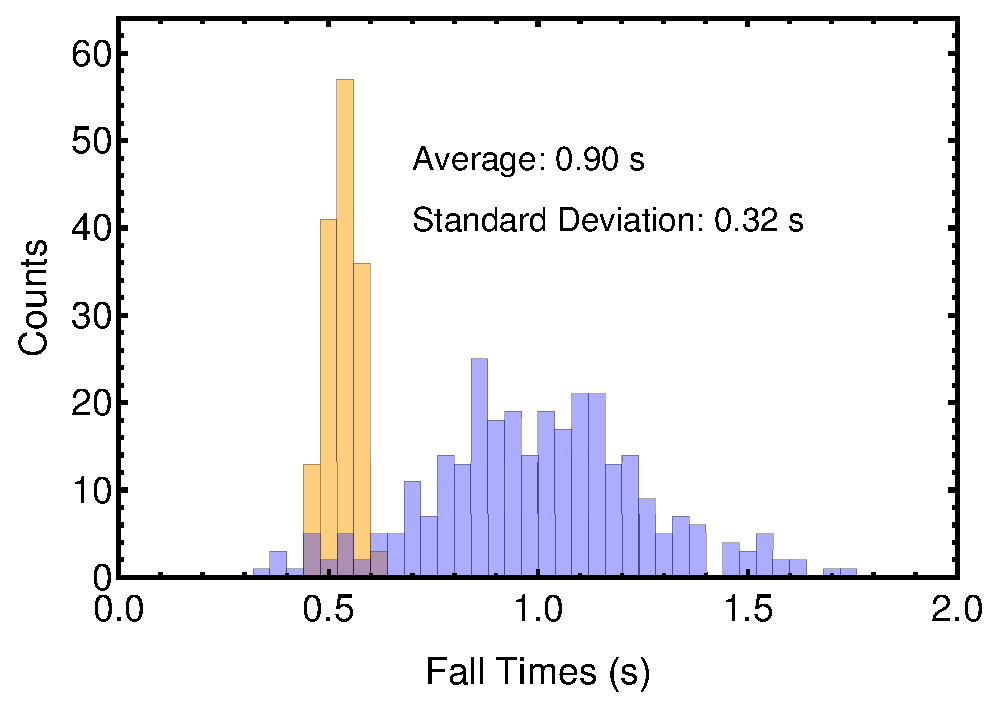
\includegraphics[height=2.25in]{measurement_uncertainty/histogram_color.eps}\label{SampleHist1}
\index{color page}
\end{figure}

(f) What advantages do histograms have over just calculating the average and standard deviation?
\answerspace{20mm}

\textbf{Homework} 

1. Suppose you made the following five length measurements of the width of a
piece of $8\frac{1}{2} {}''\, \times 11''$ paper which has been cut carefully by
a manufacturer using an unfamiliar centimeter rule: 21.33 cm, 21.52 cm, 21.47
cm, 21.21 cm, 21.45 cm. (a) Find the mean and standard deviation of the measurements.
The formal mathematical definition of standard deviation 
is given in Appendix \ref{treatment}. 
\answerspace{30mm}

\pagebreak[2]
(b) Is there any evidence of uncertainty in the measurements or are they precise?
Explain. 
\answerspace{20mm}

(c) Is there any evidence of systematic error in the measurements? If so, what
might cause this? Explain.
\answerspace{20mm}

2. Suppose Ashley and Ryan each throw darts at targets as shown below. Each
of them is trying very hard to hit the bulls eye each time. Discuss in essay
form which of the two students has the least amount of random
error associated with his
or her throws and is thus more precise. Is one of the students less accurate
is the sense of having a systematic error associated with his or her throws?
What factors like eyesight and coordination might cause one to be more precise
and another more accurate?

\vspace{0.3cm}
{\par\centering 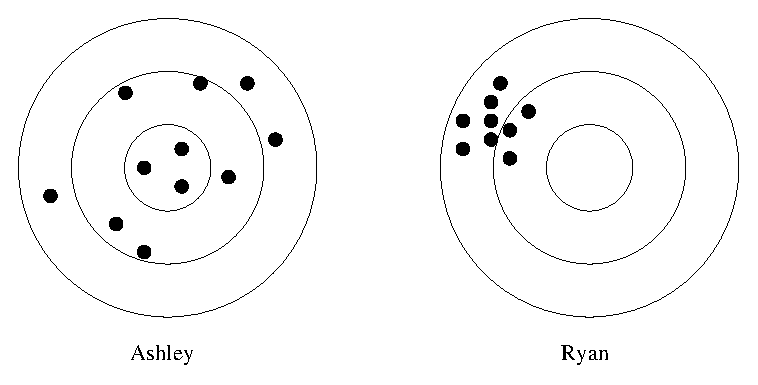
\includegraphics{measurement_uncertainty/measurement_uncertainty_fig1.eps} \par}
\vspace{0.3cm}

